\documentclass[11pt]{article}
\usepackage[paper=letterpaper,margin=1in]{geometry}
\usepackage{subfig}
\usepackage{graphicx}
\usepackage{fancyvrb}
\usepackage{upquote}
\usepackage[colorlinks=true, linkcolor=blue, urlcolor=blue, citecolor=blue, anchorcolor=blue]{hyperref}
\usepackage{amsmath}
\usepackage[siunitx]{circuitikz}
\usepackage{indentfirst}
\usepackage{fancyhdr}
\usepackage{titling}
%NOTE: Define Author, Title AFTER this package is imported.
\fancypagestyle{myfancy}{
\fancyhead[L]{\theauthor}
\fancyhead[C]{\thetitle}
\fancyhead[R]{\thepage}
\fancyfoot[C]{}
}
\pagestyle{myfancy}

\title{CS 484 Final Project: Simon Game}
\author{Brandon Ingli}
\date{\today}

\begin{document}

\maketitle

\section{Circuitry}

\begin{figure}[h]
  \centering
  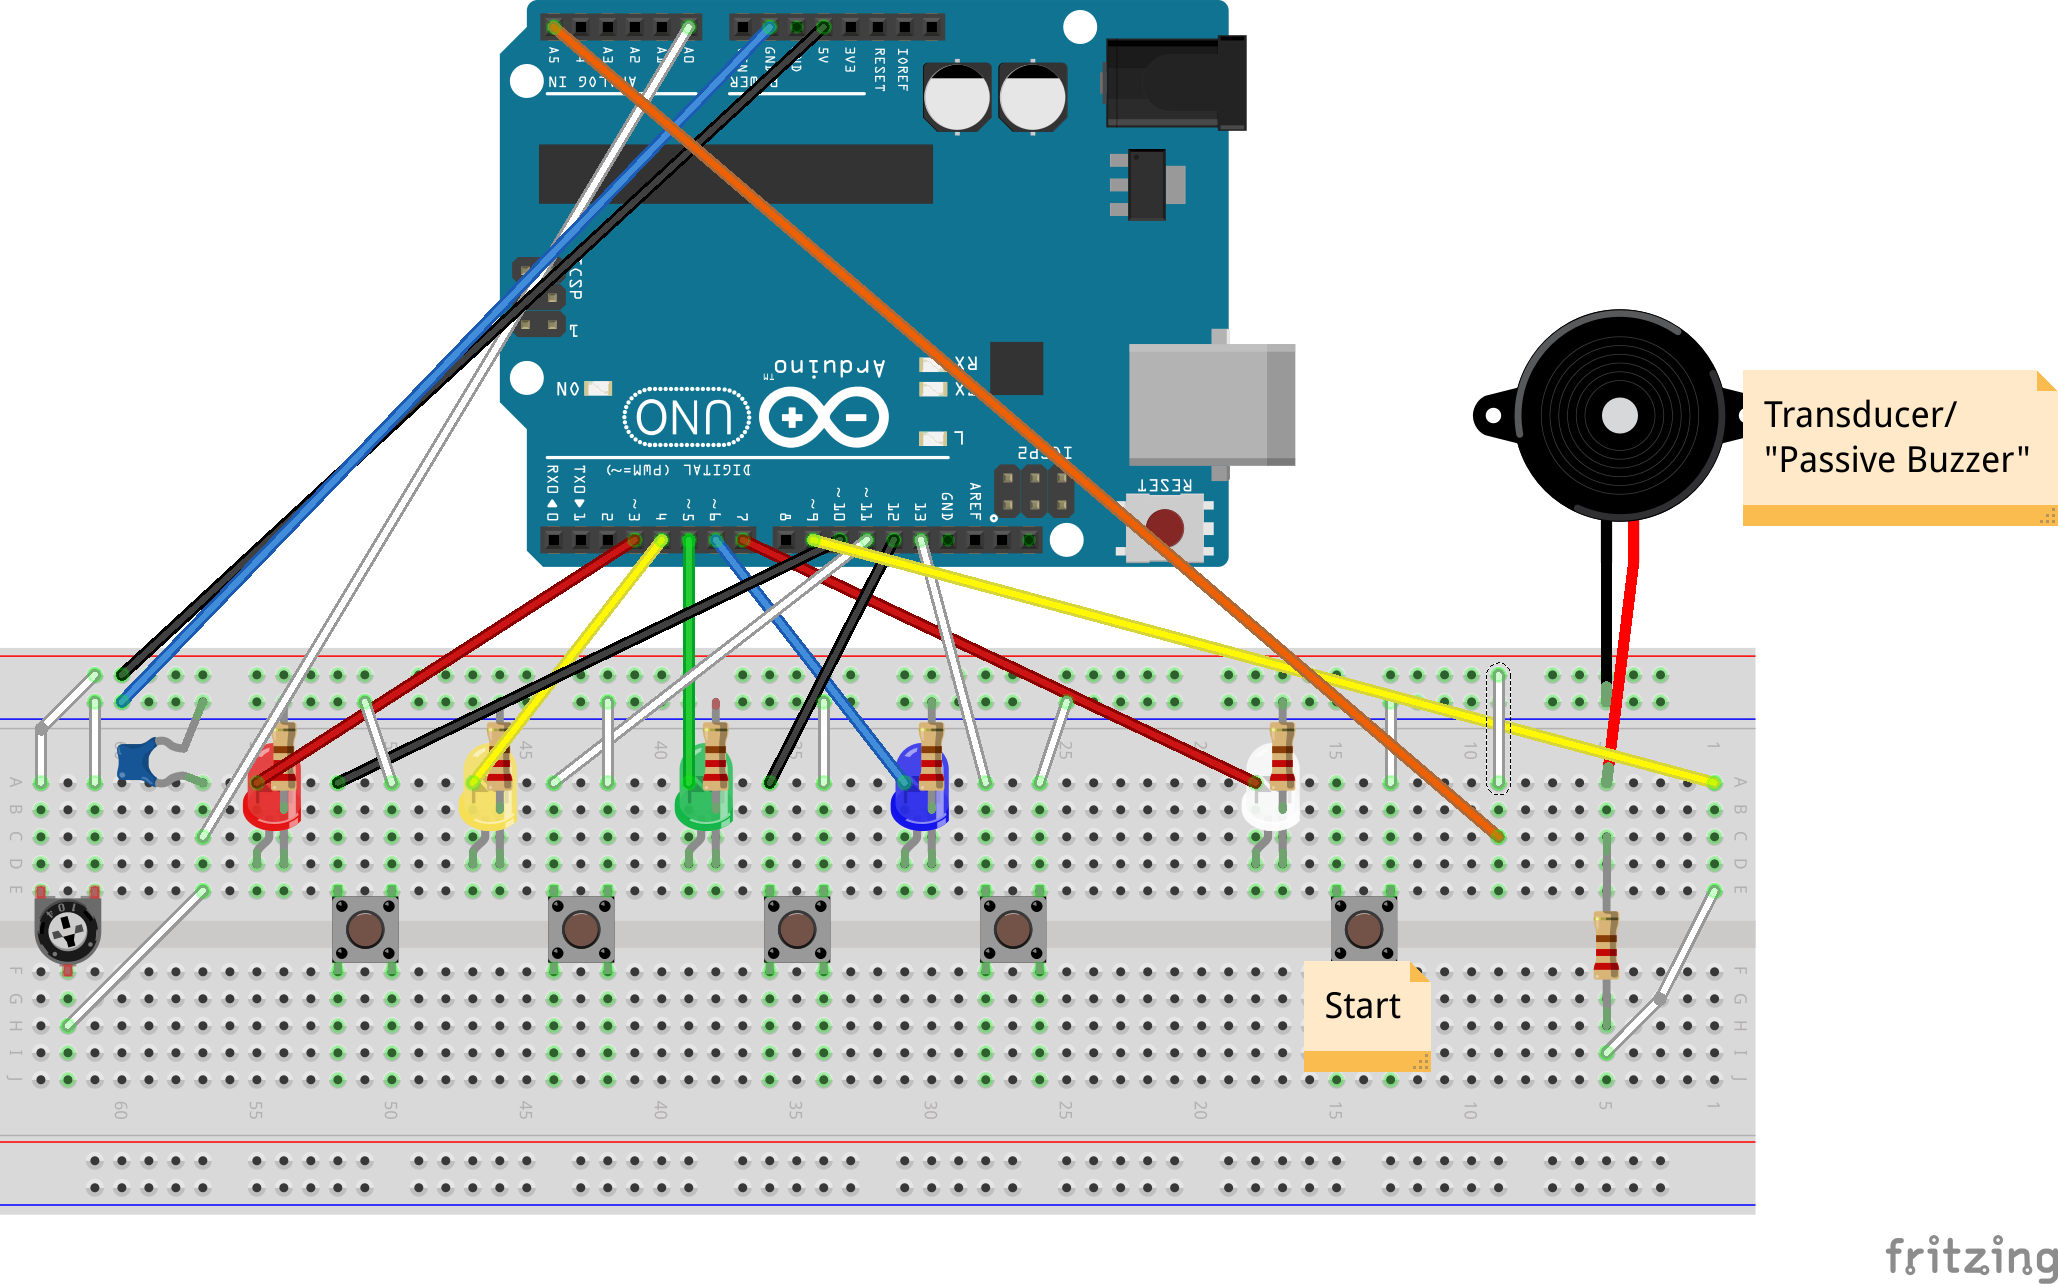
\includegraphics[width=\textwidth]{simon_game.png}
  \caption{Simon Game Breadboard}
  \label{fig:breadboard}
\end{figure}

A graphic representation of my breadboard setup can be found in figure \ref{fig:breadboard} 
on page \pageref{fig:breadboard}. There are five identical sets of LEDs (with 
220\si{\ohm} current-limiting resistors) and grounded buttons. The LEDs are wired 
to pins \texttt{PD3} to \texttt{PD7}. The buttons for the gameplay are wired to 
\texttt{PB2} to \texttt{PB5}, and the start button is wired to \texttt{PB1}. All 
button pins have their internal pull-up resistors enabled.

Pin \texttt{PC1} is used as a debug switch. Before every game, this is checked to 
see if debugging should be enabled or not. Setting the pin high enables 
debugging, and grounding it disables debugging. Again, this debug state is only 
checked and changed when a new game begins

A potentiometer is present wired between ground and 5\si{\volt}, with the wiper 
attached to pin \texttt{PC0} in parallel with a 100\si{\nano\farad} capacitor. This 
potentiometer will be used to seed the RNG. There is no capacitor from \texttt{AREF} 
to ground.

The buzzer is wired from \texttt{PB1}, through a 220\si{\ohm} resistor to bring down 
the volume, and then through the buzzer to ground.

\section{Rules and Gameplay}
\begin{enumerate}
  \item Press ``Start'' (\texttt{PB1}) to wake the microcontroller from sleep and start the game. 
        The welcome animation and jingle (from Super Mario) will play.
  \item Watch and remember the sequence. If debugging is enabled, the added item will be sent over 
        UART Serial at 9600 baud.
  \item When the white LED turns on, start repeating the sequence. When a button is pressed, the corresponding 
        LED will light and the appropriate buzzer tone will sound. Once the buzzer turns off and that LED 
        extinguishes, enter the next element in the sequence. Once the white LED turns off, the sequence 
        is complete. If 30 seconds pass between button presses, the game ends.
  \item Repeat while you correctly recall the sequence.
  \item When you incorrectly enter an element in the sequence, the game ends. A buzzer will sound and all 
        LEDs will extinguish to acknowledge this. You score will be reported by lighting/sounding yellow 
        for every hundred, green for every ten, and blue for every one element in your score. The score 
        will also be sent over UART Serial if debugging is turned on.
  \item The goodbye animation and jingle (also from Super Mario) will play, and the microcontroller 
        will go to deep sleep.
  \item If you pass 250 items, the super mario jingle will play, your score will be counted, and the microcontroller 
        will go to deep sleep.
  \item Press ``Start'' again to start a new game.
\end{enumerate}

\section{Implementation Choices}
\subsection{PWM}
I decided to use Timer 1 for PWM. The 16-bit counter allows for me to generate 
PWM frequencies within easy human hearing. I decided to look up frequencies for 
musical notes, and with a frequency divider of one, created an array of \texttt{TOP} 
values to create one octave of the c-major scale. My buzzer library allows for 
easy changing of \texttt{TOP} value (and corresponding match value for a 50\% 
duty cycle) by selecting notes 0 through 7 of the scale, or by supplying a custom 
\texttt{TOP} value to create another note.

\subsection{Button Debounce}
I chose to debounce my buttons in software, mainly because I do not have the hardware 
to do so. I have timer 2 running and overflowing at about 61\si{\hertz}. If a button is 
polled as being held for four interrupts in a row, a flag is set that the stored button 
value is correct, at which point the program continues. The start button is not 
debounced, as I feel it unnecessary. Upon first contact, \texttt{INT0} is disabled 
anyway, meaning bounce will not affect the program at all. Even if I did not immediately 
disable this particular interrupt, the ISR is empty, so the only ill effect would 
be a temporary delay in the program.

Timer 2 was chosen over timer 0 for two reasons. First, I wanted an excuse to 
learn more about the slight differences for timer 2, including the different 
timer divider options. Additionally, timer 2 can run at the \texttt{PWR\_SAVE} 
power state, deeper than timer 0. This allows me to put the processor to sleep 
while waiting for the next button poll interrupt instead of running a busy 
loop.

\subsection{Timeout}
The timer 2 polling also serves as the timeout mechanism. At each interrupt, a 
time remaining counter, which is initialized to the timer 2 frequency times the 
desired timeout in seconds, is decremented. When a button is detected to be 
pressed, this counter resets to its maximum value. Should the timeout counter 
hit zero, the button pressed is set to \texttt{0xff} --- a button that doesn't 
exist --- and the flag that the button value is correct is set. Therefore, 
the game treats it as though you pressed an incorrect button. This behavior is 
excellent, as it properly closes out the game and sets the microcontroller to 
deep sleep.

\subsection{Debugging}
I decided to implement UART Serial debugging to a computer, mainly because my 
memory stinks. Without this aid, I cannot even make it to ten elements most of 
the time, so I could not accurately test the end game behavior for score $>$ 10. 
In theory, I could test a score $>$ 100, but I don't have the time to sit and 
press buttons. I did manually initialize the score over 100 to make sure the game 
behaves as expected should someone be superhuman.

As an aside, I found that the Arduino extension for Visual Studio Code is great 
for projects such as this. While I'm not using any of the Arduino-specific 
features of the extension, which aims port all the functionality of the 
Arduino IDE into VSC, the extension also includes a serial monitor. Selecting 
the serial port, baud rate, and opening/closing the monitor can all be done 
from the VSC control pallette. While using VSC, I did have to turn off 
error squiggles for C within the workspace, since I couldn't get the AVR specific 
packages recognized no matter what I did. To disable these, put \texttt{"C\_Cpp.errorSquiggles": "Disabled"} 
in the workspace settings.
  
\end{document}